\documentclass[12pt,fleqn]{article}\usepackage{../../common}
\begin{document}
Ders 2

Bir soruyla ba�layal�m: e�er yer�ekimi kuvveti ve elektrik kuvveti kavga
etse kim yenerdi?

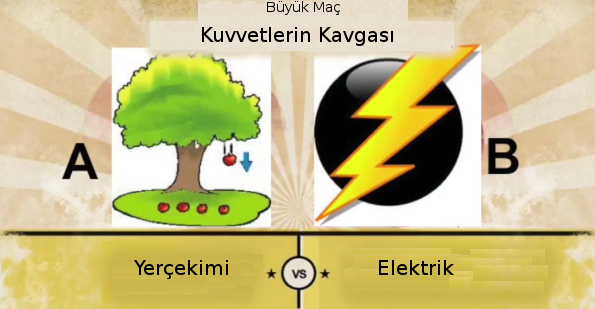
\includegraphics[width=20em]{02_01.png}

[Hoca bu soruya cevab� s�n�f i�i oy verme sisteminde sordu, oylar geldi,
87\% elektrik dedi]. Tamam. �imdi bu sorunun cevab�n� bilimsel olarak
vermeye u�ra�aca��z. Matematik ve mant�k kullanarak cevab� bulmaya
u�ra�aca��z.  

Kavgan�n tabii ki kurallar� olmal�, ki adil bir kap��ma olsun. 

Kap��man�n yeri olarak bir hidrojen atomunu se�ece�iz. Hidrojen atomi bir
proton ve bir elektrondan olu�ur, bu ikisi aras�nda �zel bir mesafe
oldu�unu varsayaca��m, ve bu mesafe �zerinden bu iki ��e aras�nda hem
yer�ekimi, hem de elektrik kuvvetini hesaplayaca��m. 

















\end{document}
















